% !TEX TS-program = pdflatex
% !TEX encoding = UTF-8 Unicode
% Version of 08-Jun-2011

\documentclass[letterpaper,12pt]{article}

% setup page dimensions
% read geometry.pdf for detailed page layout information
\usepackage[margin=0.75in, letterpaper]{geometry} 

% favorite packages
\usepackage{graphicx}        % import graphics
\usepackage{subfig}          % multiple images in figs
\usepackage{textcomp}        % Greek in text mode - \textmu
\usepackage{hyperref}        % urls - \href{url}{text}
\usepackage{verbatim}        % adds environment for commenting out blocks of text & for better verbatim
\usepackage[parfill]{parskip} % Activate to begin paragraphs with an empty line rather than an indent

% define degree symbol
\newcommand{\degree}{\ensuremath{^\circ}}

% define commands for subscripts & superscripts to use in text mode
\newcommand{\superscript}[1]{\ensuremath{^{\textrm{#1}}}}
\newcommand{\subscript}[1]{\ensuremath{_{\textrm{#1}}}}

% The preamble for this document...
\title{Analysis of radioisotope wipe samples using the Tennelec LB5500 spectrometer}
\author{John R. Minter and Craig S. Swanson}
\date{May 11, 2012}


\begin{document}


\begin{center}
\Large{
\textbf{
Analysis of radioisotope wipe samples \\
using the Tennelec LB5500 spectrometer \\
Report of Analysis}
}
\vskip 0.125in
\normalsize{
   \begin{tabular}{r l}
   \textbf{Job Report No.:}       & QM12-04-01 \\
   \textbf{Client:}               & John Heyer  \\
   \textbf{Responsible Analysts:} & Craig Swanson  \\
                                  & John Minter \\                        
   \textbf{Date:}                 & May 11, 2012 (ammended)  \\
   \textbf{Charge number:}        & 11137  \\
   \end{tabular}
}
\end{center}

\section*{Abstract}
Filter wipe samples are collected semi-annually to check
for radiation contamination of sealed radioactive sources by
leakage. The activity of these samples is determined by using
an alpha/beta gas proportional counter. Results are used to
insure the safety of Kodak employees and to meet the requirements
set by the New York State Department of Environmental
Conservation.

Here we report the results from 142 wipe samples supplied
by Linda Reibsome over the period from April 5, 2012 to May 8, 2012.

Note that in this analysis, three samples were numbered with the wrong
accession number (3015, 3016, and 3029)  in batch 2751 in the Eclipse
software. Two of the envelopes were mis-labeled with the wrong accession
number (132, and 3756.) These errors were manually corrected in the final
.csv file with the approval of the client.


\section*{Introduction}
Filter wipe samples are collected to check for radiation
contamination of sealed radioactive sources for leakage.
The activity of these samples is determined by using an
alpha/beta gas proportional counter. Results are used to
insure the safety of Kodak employees and to meet the requirements
set by the New York State Department of Environmental
Conservation. 

The objective of this report is to document the analysis
from Spring 2012.

\subsection*{Range and Sensitivity}
The method can detect a wide range of activity.  Most samples
collected in this manner have low activity level. The lower limit
is determined by measuring blanks with each set of samples. Recent
blanks have both alpha and beta maximum activities below 10 pCi.

\section*{Results Summary}
The full list of results from individual wipes is attached as
a comma-delimited file, easily imported and sorted with Excel.
A summary of the results is shown in the table below

\begin{center}
   \begin{tabular}{| r | r | r | r | r | r | r |}
   \hline
   \textbf{Meas.}                  &  Min. &  1Qu  & Median & Mean   &  3Qu   &   Max.  \\
   \hline
   \textbf{Blanks  $\alpha$ [pCi]} & 0.380 & 0.507 & 0.634  & 1.155  & 0.887  & 4.690  \\
   \hline
   \textbf{Blanks  $\beta$ [pCi]}  & 1.658 & 1.842 & 2.118  & 2.824  & 2.579  & 8.289 \\
   \hline
   \textbf{Samples $\alpha$ [pCi]} & 0.127 & 0.761 & 1.648  & 22.280 & 10.580 & 936.100 \\
   \hline
   \textbf{Samples $\beta$ [pCi]}  & 1.197 & 2.210 & 2.763  & 5.980  & 4.237  & 156.500   \\
   \hline
   \end{tabular}

\end{center}

\subsubsection*{Detector efficiency}
The detector efficiency for  Am-241
( 95\% confidence interval = $0.3586\pm 0.00069$ for $n=9$)
and Cl-36
( 95\% confidence interval = $0.4935\pm 0.0022$ for $n=9$)
are shown below in
Figures ~\ref{ana:Am} and ~\ref{ana:Cl}. 

\begin{figure}[h!]
\begin{center}
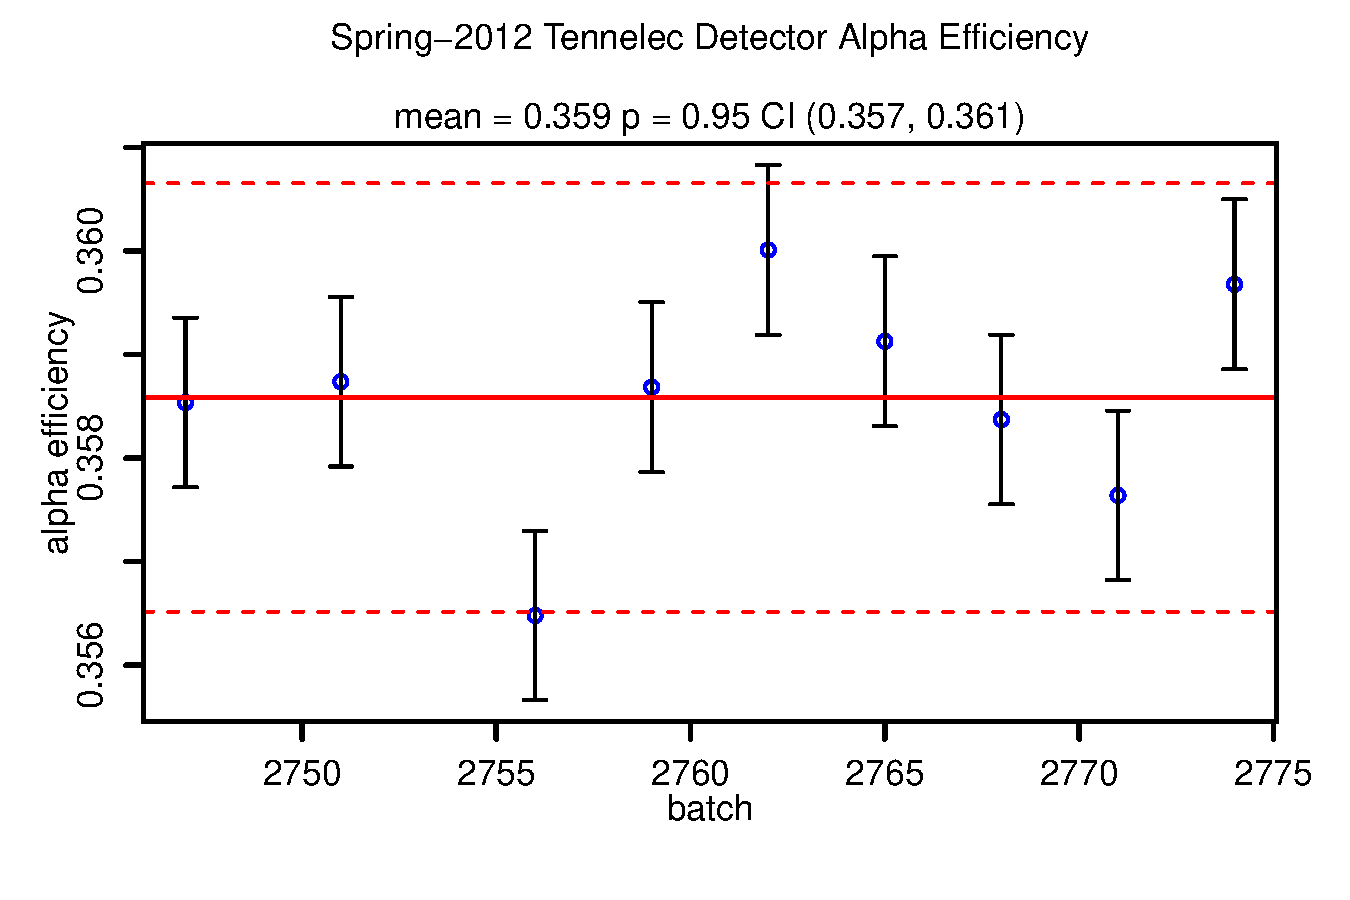
\includegraphics[width=0.75\textwidth]{./figs/Spring-2012-alpha-efficiency.pdf}
\end{center}
\caption{Detector alpha efficiency}
\label{ana:Am}
\end{figure}

\begin{figure}[h!]
\begin{center}
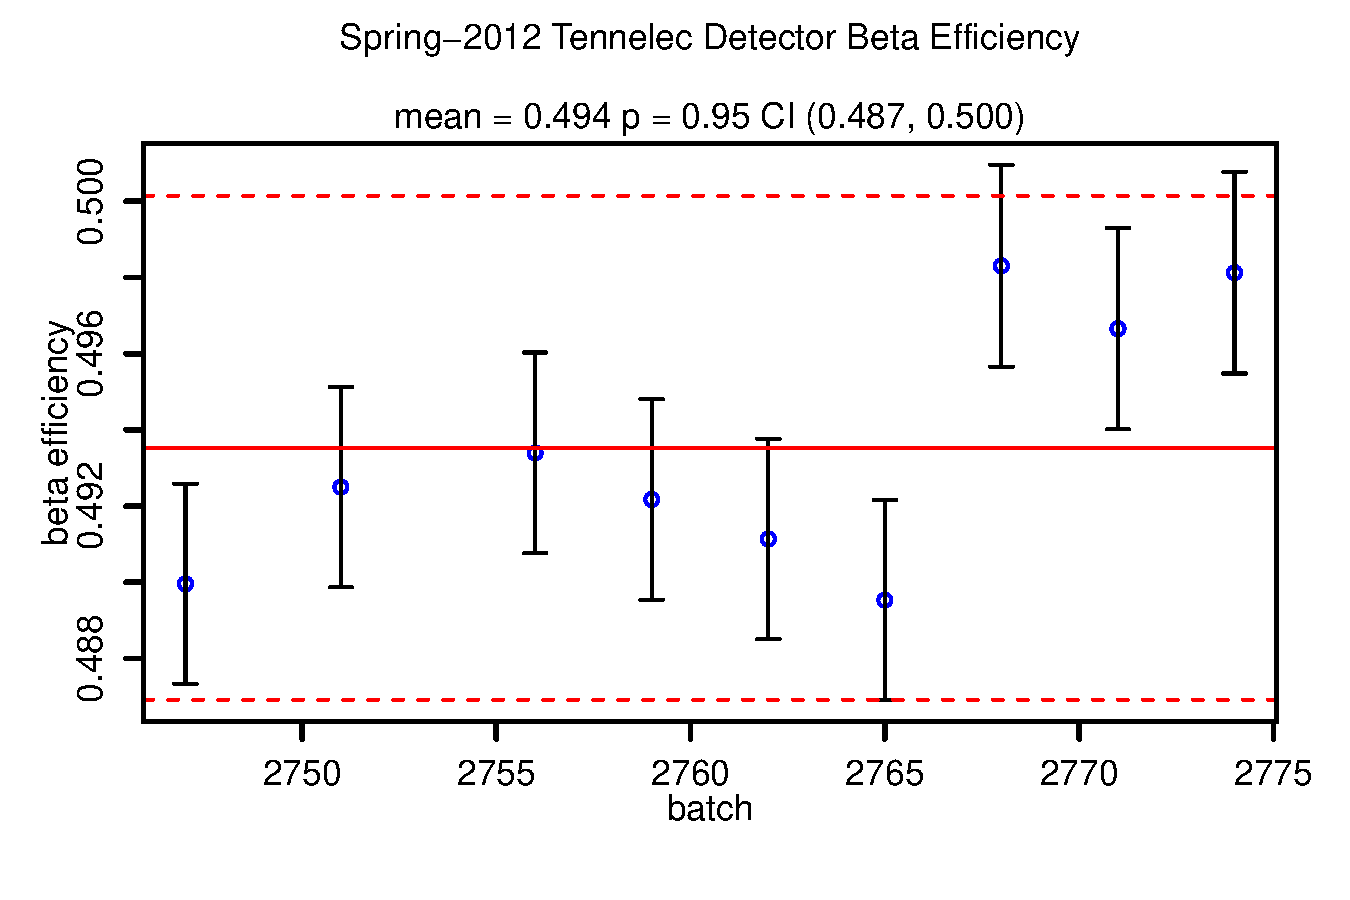
\includegraphics[width=0.75\textwidth]{./figs/Spring-2012-beta-efficiency.pdf}
\end{center}
\caption{Detector beta efficiency}
\label{ana:Cl}
\end{figure}


\section*{Materials and Method}

\subsection*{Standards}
Two NIST-traceable radioactive sources of known activity are analyzed
with each set of samples to determine the counting efficiency of the
instrument. Currently, these include a CM-36 beta standard
(Source RR-659, certified on Jan. 13, 2000) and an Am-241 alpha standard
(Source 170-94, certified on Sep. 11, 1986).

\subsection*{Sample and Mounting}

Samples and Blanks are supplied by a contractor on Whatman \#1 qualitative
filter paper or equivalent for performing wipe tests. The samples are submitted in
small manila envelopes sample storage. Each envelope is labeled with the source
accession number and the date sampled.

The sample filter is removed from the envelope with forceps, exposed side up,
and mounted on a planchet in the center of a numbered Tennelec LB5500
sample holders.

\subsection*{Spectrum Acquisition}
At the beginning of each batch of samples, a blank and two check standards
(alpha and beta) are loaded into their numbered sample holders. These are combined
with the samples mounted in their numbered sample holders.

The analyst creates a  ``Batch'' file must in the Eclipse software that
controls the Tennelec LB5500. The analyst does this by selecting
``manage'' from the pull-down menu at the top of the window, then selecting
``samples'', and clicking on ``new''. The analyst enters (and records) a
numeric batch ID and sets the procedure to ``smear''. The analyst enters
the sample ID (the Kodak accession number of the source tested or the
standard ID) in the ``lab ID'' field. 

When finished, the analyst saves and prints the batch file.

Finally, the analyst runs the batch by going to the ``count''
pull-down menu and selecting ``Go''. This causes each sample to be
counted for ten minutes.


\subsection*{Spectrum Analysis}

The Tennelec ``Eclipse'' software stores the results
from running their stored procedures in a Microsoft Access
database (``Eclipse.mdb'') that is stored in the program directory
on the control PC. A backup copy of this file is stored on a network
file share after each semi-annual analysis is complete. This provides
sufficient archival storage.

\subsection*{Data Reduction and Report Generation}

All the data required for data reduction and report generation is
stored in the ``Eclipse.mdb'' database and may be automatically
retrieved and analyzed a custom script written using the Open Source
R Statistical Programming language (``wipeTest.R'').

The analyst simply edits title of the report and the vector of batch
numbers to match batches in the Tennelec database. The analyst has the
option of computing the efficiency using the standards from the batch
file -- an option we chose to use because of the large number of batches,
or to use recent results which is appropriate for analysis of a few
retests. 

The module then retrieves all the data, computes and plots the mean detector
efficiency for alpha and beta radiation if the option was selected,
processes all the raw data, and outputs summary statistics and a
results file sorted by accession number.






\end{document}
